%\begin{figure*}[t!]
%	\centering
%	\subfloat[Heavy hitter analysis]{
%		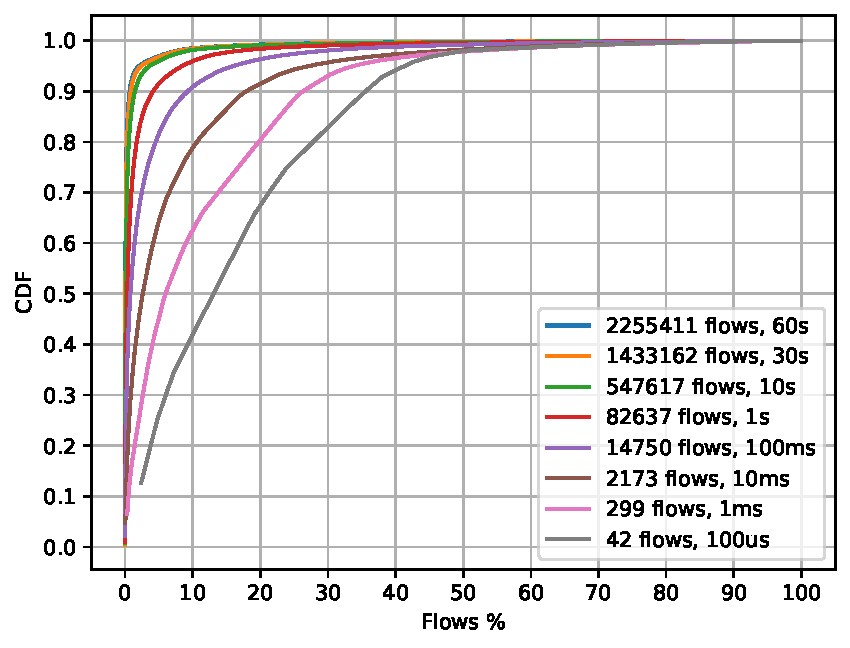
\includegraphics[width=0.33\textwidth]{fig_cdf.pdf}
%		\label{fig:cdf}
%	}
%	\subfloat[Flow duration]{
%		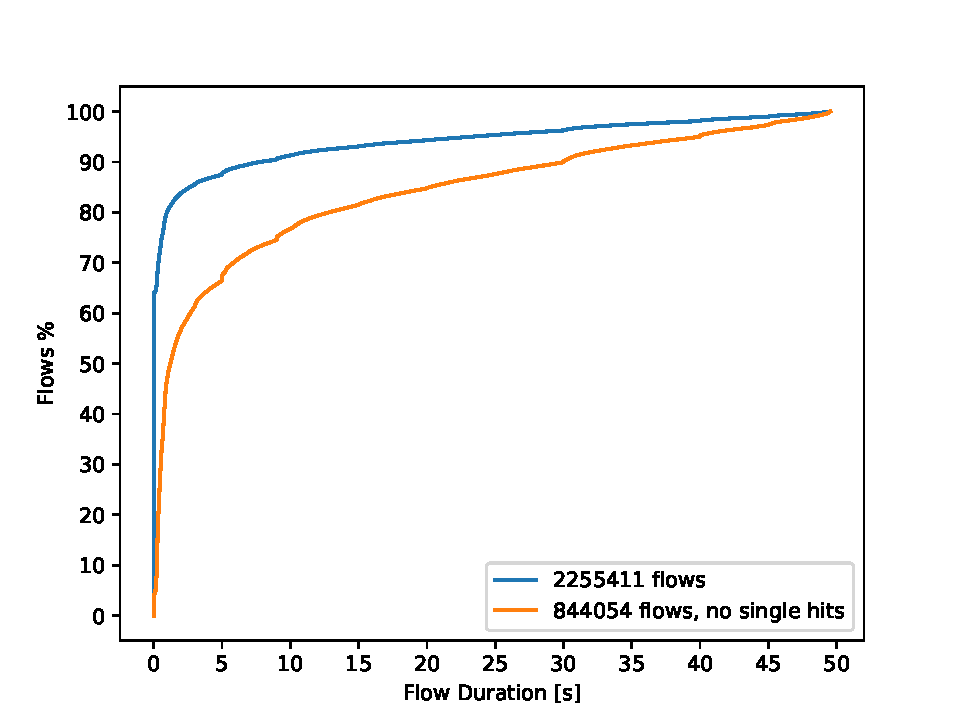
\includegraphics[width=0.33\textwidth]{fig_duration.pdf}
%		\label{fig:flow_duration}
%	}
%	\subfloat[Average flow size]{
%		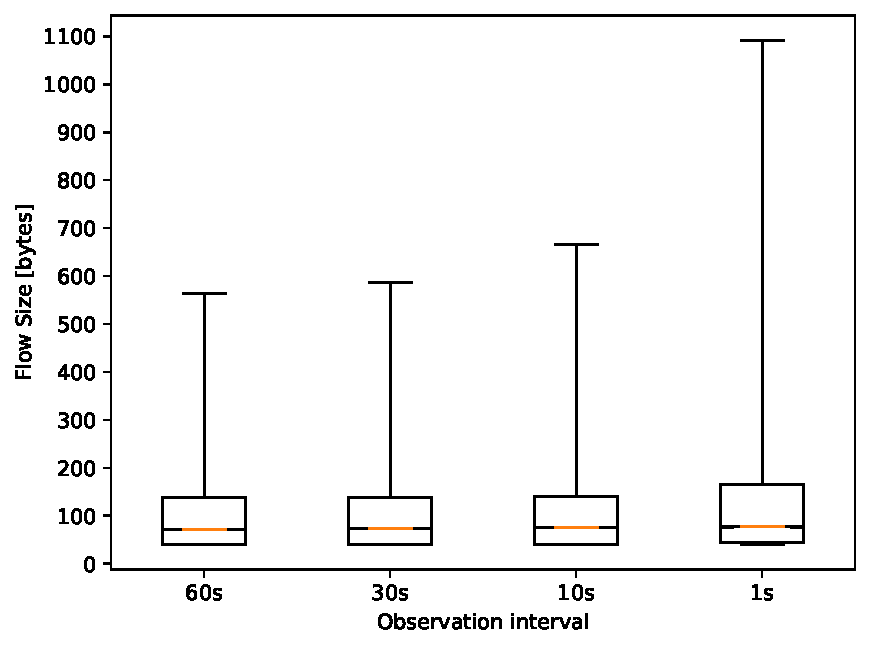
\includegraphics[width=0.33\textwidth]{fig_avg_flow_size.pdf}
%		\label{fig:flow_size}
%	}
%	\caption{CAIDA trace summary}
%	\label{fig:traces}
%\end{figure*}

\section{Learning from the Traffic}\label{sec:traffic}

Network traffic has been observed to follow a Zipf distribution as a few network flows account for most of the whole network traffic~\cite{Sarrar:2012,Jin:2017}.

In our study, we conducted experiments to determine the traffic characteristics of an up-to-date real-world data center trace.
We replayed a CAIDA network trace extracted from an IXP in a data center in New York dated from January 2019~\cite{caida:19}.
The analysed trace is 1 minute long monitoring $\sim$\SI{30}{\mega\nothing} packets in a full-duplex \SI{40}{\giga\bit/\second} Ethernet link connecting New York and S\~ao Paulo/Brazil.
A similar analysis was done by~\citeauthor{Spang:19} to estimate the number of TCP/IP flows~\cite{Spang:19}.

Figure~\ref{fig:traces} summarizes our observations.
In our analysis, we defined a flow as being a unique five-tuple $\langle$~IPv4/IPv6 Source IP address, IPv4/IPv6 destination IP address, L4 protocol, UDP/TCP source port, UDP/TCP destination port~$\rangle$ connection.

As shown in Figure~\ref{fig:cdf}, the Zipf distribution characteristic is still present in current network traffic.
The figure presents the CDF, in terms of transmitted bytes, for several observation intervals, ranging from \SI{100}{\micro\second} to \SI{60}{\second}.
For all observation intervals longer than \SI{100}{\milli\second}, fewer than 10\% of the flows dominate more than 90\% of the traffic.
For shorter intervals, the Zipf dominance is still present although more skewed.

Figure~\ref{fig:flow_duration} presents the flow duration time.
The blue curve is dominated (60\%) by single packet flows.
Single packet flows are represented with a flow duration of zero seconds.
Short-lived flows dominate the trace with $\sim$90\% of all flows lasting less than 5 seconds.
The orange curve in Figure~\ref{fig:flow_duration} illustrates the duration of flows with multiple hits in the trace.
Still, short-lived flows dominate the trace with $\sim$50\% lasting less than 1 second in the trace.

Figure~\ref{fig:flow_size} presents the average flow size for four statistically representative observation intervals.
For all four measures, the first quartile, the median, and the third quartile are very similar.
On average, small flows ($\sim$100 bytes) dominate the trace with 75\% of the flows being no larger than 150 bytes.

According to our experiments, the expected Zipf distribution characteristic of network traffic is still present in current data center traffic.
Such characteristic favors flow caching in memory scarce programmable dataplanes.
However, we notice that short-lived flows dominate the trace.
Therefore, the chosen cache policy algorithm needs a fast reaction time to quickly adapt to traffic changes.
Besides, such temporal traffic characteristic possibly favors time-aware cache policies (e.g. LRU).

\section{Cache Replacement Algorithms}\label{sec:policies}

\subsection{Cache Eviction Policies}

\textbf{OPT}~---~The optimal (OPT) replacement policy~\cite{Belady:66} is an oracle algorithm that relies on knowing the future traffic behavior.
OPT uses this information to replace data that is further referenced in time.
Due to that, OPT is not realistically implementable and it is commonly used to evaluate cache performance since it sets an upper performance bound for realistic caching systems.

\textbf{Random}~---~Random or pseudo-random replacement policies use a stochastic random function to select a victim for eviction.
Pseudo-random cache policy has been widely adopted in ARM-based processors.
In random policies, no history on cache misses/hits nor cache access frequency is required.
The efficiency of a random policy is directly related to the quality of its random generator function.

\textbf{LRU}~---~The LRU replacement algorithm evicts the most ancient cache entry in case of a cache miss.
A possible LRU implementation uses a timestamp tag to sort cache entries by recency, as in Algorithm~\ref{algo:lru}.

\begin{algorithm}[]
	\caption{LRU policy}
	\label{algo:lru}
	\SetInd{0.1em}{.9em}
	\SetAlgoLined
	\footnotesize
	\SetKwProg{procedure}{Procedure}{}{end}
	\SetKwFunction{minTimestampEntry}{minTimestampEntry}
	\SetKwFunction{findEntry}{findEntry}
	\SetKwFunction{lruPolicy}{lruPolicy}
	\SetKwInOut{Input}{input}
	\SetKw{In}{in}%
	\SetKw{Not}{not}%
	\SetKw{Or}{or}%
	\SetKw{Continue}{continue}%
	\SetKw{True}{true}%
	\Input{Cache memory: list of $\langle$\texttt{entry, timestamp}$\rangle$ pairs}
	\Input{Possible cache entry}
	\Input{Packet timestamp}
	\procedure{\lruPolicy{cache, possible\_entry, current\_timestamp}}{
		\If(\hfill\tcp*[h]{Cache hit}){possible\_entry \In cache}{
			entry\_found =  \findEntry{cache, possible\_entry}\hfill\tcp{Hit pointer}
			entry\_found$\rightarrow$timestamp  = current\_timestamp
		}
		\Else(\hfill\tcp*[h]{Cache Miss}){
			victim = \minTimestampEntry{cache}\hfill\tcp{Victim pointer}			
			*victim = $\langle$possible\_entry, current\_timestamp$\rangle$
		}
	}
\end{algorithm}

\textbf{LFU}~---~Contrarily to LRU, LFU uses hit frequency rather than the access time to evict entries.
LFU uses a frequency counter to sort cache entries by frequency.
In case of a hit, the frequency counter is incremented.
Otherwise, the cache entry with the lowest frequency is chosen for eviction, as in Algorithm~\ref{algo:lfu}.

\begin{algorithm}[]
	\caption{LFU policy}
	\label{algo:lfu}
	\SetInd{0.1em}{.9em}
	\SetAlgoLined
	\footnotesize
	\SetKwProg{procedure}{Procedure}{}{end}
	\SetKwFunction{lfuPolicy}{lfuPolicy}
	\SetKwFunction{findEntry}{findEntry}
	\SetKwFunction{minFrequencyEntry}{minFrequencyEntry}
	\SetKwInOut{Input}{input}
	\SetKw{In}{in}%
	\SetKw{Not}{not}%
	\SetKw{Or}{or}%
	\SetKw{Continue}{continue}%
	\SetKw{True}{true}%
	\Input{Cache memory: list of $\langle$\texttt{entry, counter}$\rangle$ pairs}
	\Input{Possible cache entry}
	\procedure{\lfuPolicy{cache, possible\_entry}}{
		\If(\hfill\tcp*[h]{Cache hit}){possible\_entry \In cache}{
			entry\_found = \findEntry{cache, possible\_entry}\hfill\tcp{Hit pointer}
			entry\_found$\rightarrow$counter  += 1
		}
		\Else(\hfill\tcp*[h]{Cache miss}){
			victim =  \minFrequencyEntry{cache}\hfill\tcp{Victim pointer}
			*victim = $\langle$possible\_entry, 1$\rangle$
		}
	}
\end{algorithm}

\textbf{WLFU}~---~\textit{Vanilla} implementations of LFU perform poorly with real-world network traces~\cite{Kim:09}.
\textit{Vanilla} LFU considers all cache hits with equal weight, which is not realistic in network communications because larger packets incur in greater network efficiency compared to small ones.
Thus, Weighted LFU (WLFU) leverages \textit{vanilla} LFU by considering the packet size in its frequency counters.
A possible implementation of WLFU is illustrated in Algorithm~\ref{algo:wlfu}.

\begin{algorithm}[]
\caption{WLFU policy}
\label{algo:wlfu}
\SetInd{0.1em}{.9em}
\SetAlgoLined
\footnotesize
\SetKwProg{procedure}{Procedure}{}{end}
\SetKwFunction{wlfuPolicy}{wlfuPolicy}
\SetKwFunction{findEntry}{findEntry}
\SetKwFunction{minFrequencyEntry}{minFrequencyEntry}
\SetKwInOut{Input}{input}
\SetKw{In}{in}%
\SetKw{Not}{not}%
\SetKw{Or}{or}%
\SetKw{Continue}{continue}%
\SetKw{True}{true}%
\Input{Cache memory: list of $\langle$\texttt{entry, counter}$\rangle$ pairs}
\Input{Possible cache entry}
\Input{Packet Size}
\procedure{\wlfuPolicy{cache, possible\_entry, pkt\_size}}{
	\If(\hfill\tcp*[h]{Cache hit}){possible\_entry \In cache}{
		entry\_found =  \findEntry{cache, possible\_entry}\hfill\tcp{Hit pointer}
		entry\_found$\rightarrow$counter  += pkt\_size\hfill\tcp{Increment size counter}
	}
	\Else(\tcp*[h]{Cache miss}){
		victim =  \minFrequencyEntry{cache}\hfill\tcp{Victim pointer}
		*victim = $\langle$possible\_entry, pkt\_size$\rangle$
	}
}
\end{algorithm}

\textbf{OLFU}~---~Optmistic LFU (OLFU) is a proposition to overcome the limitations of \textit{vanilla} LFU for flow caching.
OLFU is an LFU derivation that gives a chance for a cache promotion candidate to remain in cache regardless of its \textit{actual} hit frequency.
In OLFU, the cache policer behaves as the \textit{vanilla} LFU in case of a cache hit.
Otherwise, instead of re-initializing the frequency counter, the new cache entry takes control of the victim's counter, as shown in Algorithm~\ref{algo:olfu}.

\begin{algorithm}[]
\caption{OLFU policy}
\label{algo:olfu}
\SetInd{0.1em}{.9em}
\SetAlgoLined
\footnotesize
\SetKwProg{procedure}{Procedure}{}{end}
\SetKwFunction{olfuPolicy}{olfuPolicy}
\SetKwFunction{findEntry}{findEntry}
\SetKwFunction{minFrequencyEntry}{minFrequencyEntry}
\SetKwInOut{Input}{input}
\SetKw{In}{in}%
\SetKw{Not}{not}%
\SetKw{Or}{or}%
\SetKw{Continue}{continue}%
\SetKw{True}{true}%
\Input{Cache memory: list of $\langle$\texttt{entry, counter}$\rangle$ pairs}
\Input{Possible cache entry}
\procedure{\olfuPolicy{cache, possible\_entry}}{
	\If(\hfill\tcp*[h]{Cache hit}){possible\_entry \In cache}{
		entry\_found =  \findEntry{cache, possible\_entry}\hfill\tcp{Hit pointer}
		entry\_found$\rightarrow$counter  += 1
	}
	\Else(\hfill\tcp*[h]{Cache miss}){
		victim = \minFrequencyEntry{cache}\hfill\tcp{Victim pointer}
		*victim = $\langle$possible\_entry, victim$\rightarrow$counter + 1$\rangle$\hfill\tcp{Replace reusing current counter}
	}
}
\end{algorithm}


\textbf{OWLFU}~---~To optimize cache efficiency, OWLFU combines the OLFU and WLFU cache policies.
In case of a hit, OWLFU behaves as WLFU.
Otherwise, OWLFU modifies OLFU by incrementing the current packet size to the victim frequency counter, as in Algorithm~\ref{algo:owlfu}.

\begin{algorithm}[]
\caption{OWLFU policy}
\label{algo:owlfu}
\SetInd{0.1em}{.9em}
\SetAlgoLined
\footnotesize
\SetKwProg{procedure}{Procedure}{}{end}
\SetKwFunction{owlfuPolicy}{owlfuPolicy}
\SetKwFunction{findEntry}{findEntry}
\SetKwFunction{minFrequencyEntry}{minFrequencyEntry}
\SetKwInOut{Input}{input}
\SetKw{In}{in}%
\SetKw{Not}{not}%
\SetKw{Or}{or}%
\SetKw{Continue}{continue}%
\SetKw{True}{true}%
\Input{Cache memory: list of $\langle$\texttt{entry, counter}$\rangle$ pairs}
\Input{Possible cache entry}
\Input{Packet Size}
\procedure{\owlfuPolicy{cache, possible\_entry, pkt\_size}}{
	\If(\hfill\tcp*[h]{Cache hit}){possible\_entry \In cache}{
		entry\_found =  \findEntry{cache, possible\_entry}\hfill\tcp{Hit pointer}
		entry\_found$\rightarrow$counter  += pkt\_size\hfill\tcp{Increment size counter}
	}
	\Else(\hfill\tcp*[h]{Cache miss}){
		victim =  \minFrequencyEntry{cache}\hfill\tcp{Victim pointer}
		*victim = $\langle$possible\_entry, victim$\rightarrow$counter + pkt\_size$\rangle$\hfill\tcp{Replace reusing current size counter}
	}
}
\end{algorithm}

\subsection{Cache Promotion Policies}
Describe here why the need of a cache promotion policy and which ones we studied.

\section{Evaluating Cache Perfomance}\label{sec:cache_results}

\begin{figure*}[]
\centering
\subfloat[Hit Ratio. $SF=1\times$]{
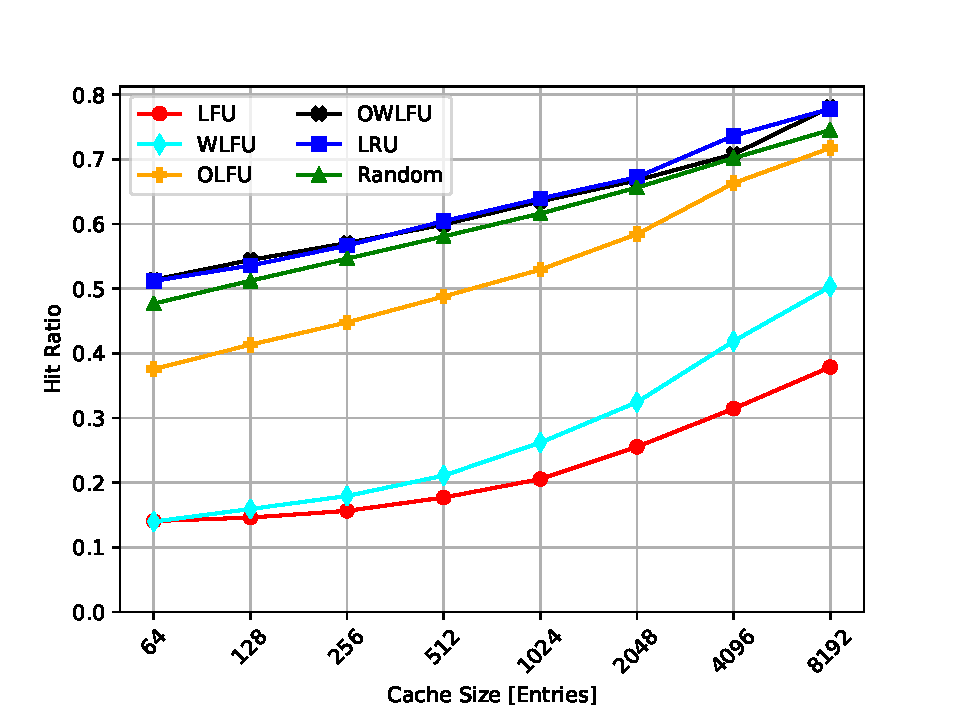
\includegraphics[width=0.33\textwidth]{hit_ratio_sf1.pdf}
\label{fig:hit_ratio_sf1}
}
\subfloat[Hit Ratio. $SF=10\times$]{
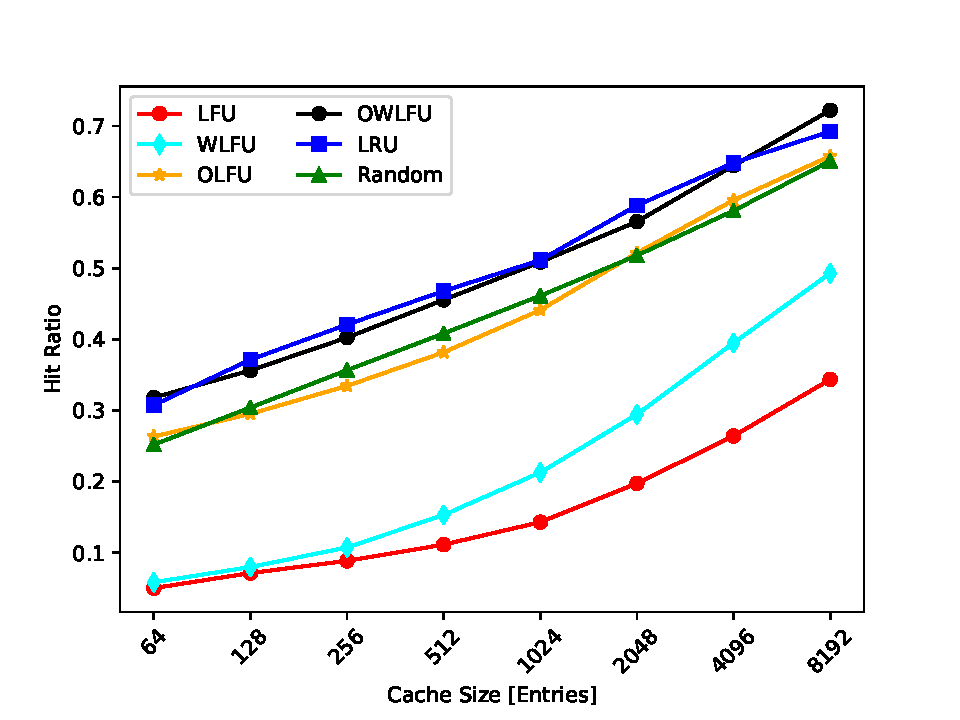
\includegraphics[width=0.33\textwidth]{hit_ratio_sf10.pdf}
\label{fig:hit_ratio_sf10}
}
\subfloat[Hit Ratio. $SF=100\times$]{
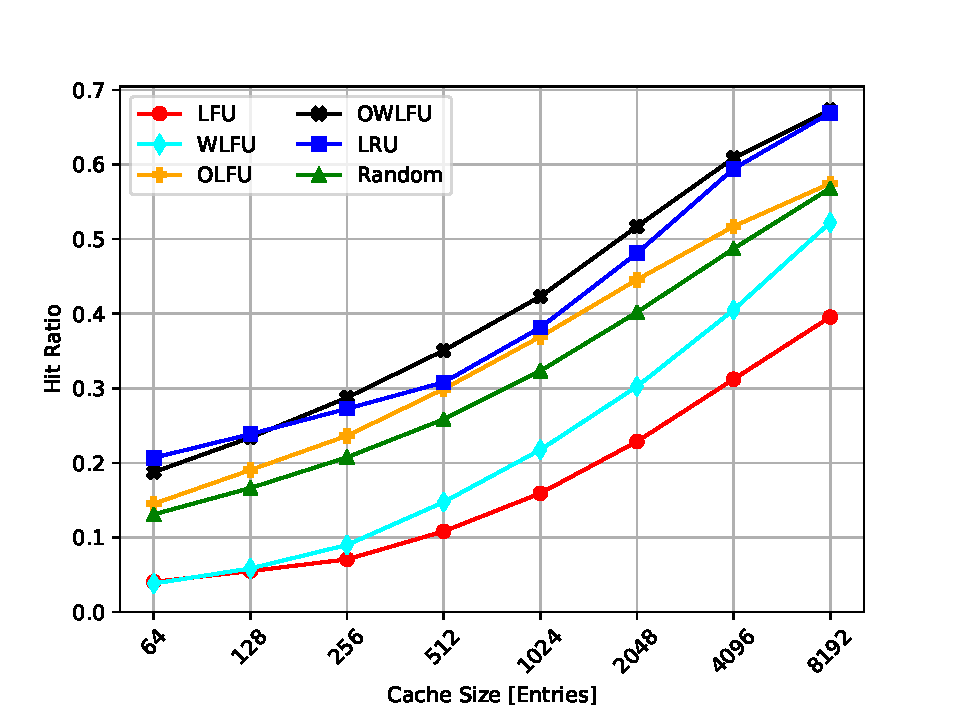
\includegraphics[width=0.33\textwidth]{hit_ratio_sf100.pdf}
\label{fig:hit_ratio_sf100}
}\\
\subfloat[Size Weighted Hit Ratio. $SF=1\times$]{
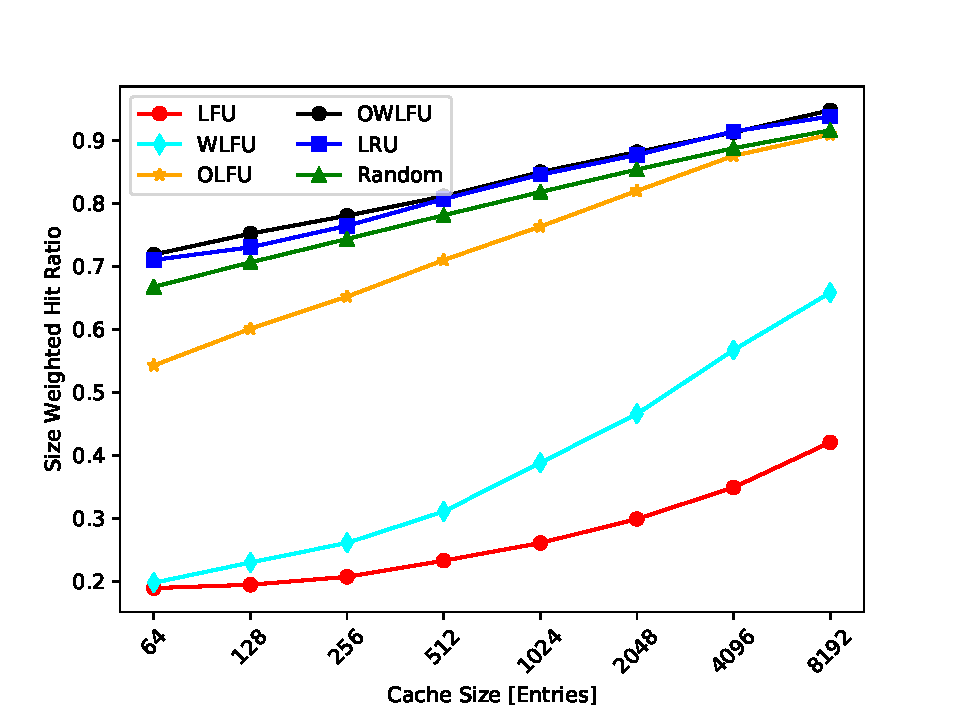
\includegraphics[width=0.33\textwidth]{weighted_hit_ratio_sf1.pdf}
\label{fig:weighted_hit_ratio_sf1}
}
\subfloat[Size Weighted Hit Ratio. $SF=10\times$]{
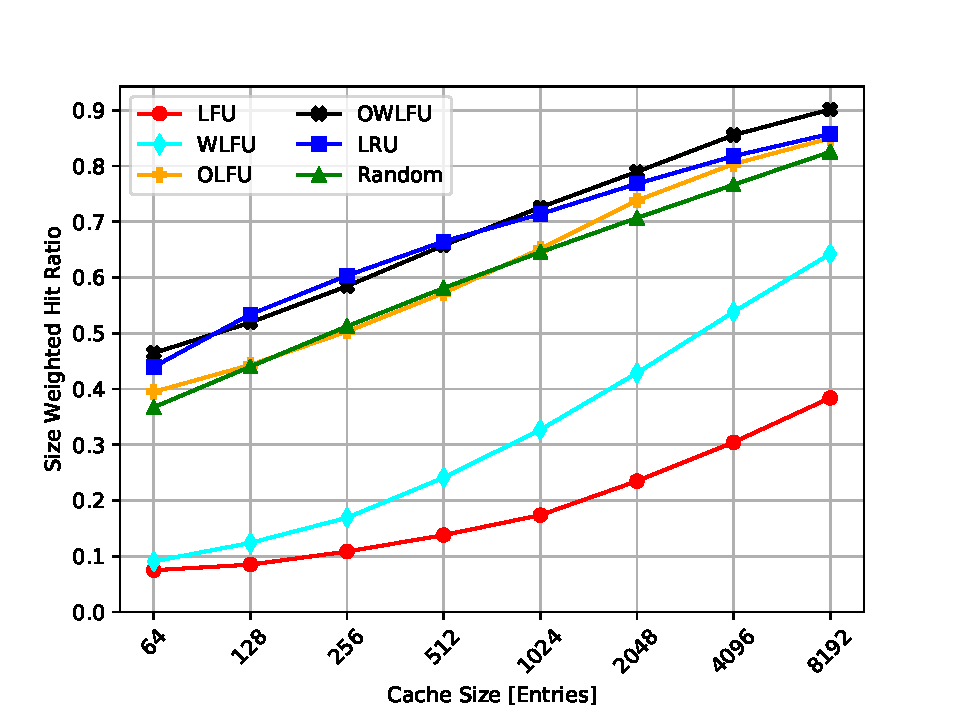
\includegraphics[width=0.33\textwidth]{weighted_hit_ratio_sf10.pdf}
\label{fig:weighted_hit_ratio_sf10}
}
\subfloat[Size Weighted Hit Ratio. $SF=100\times$]{
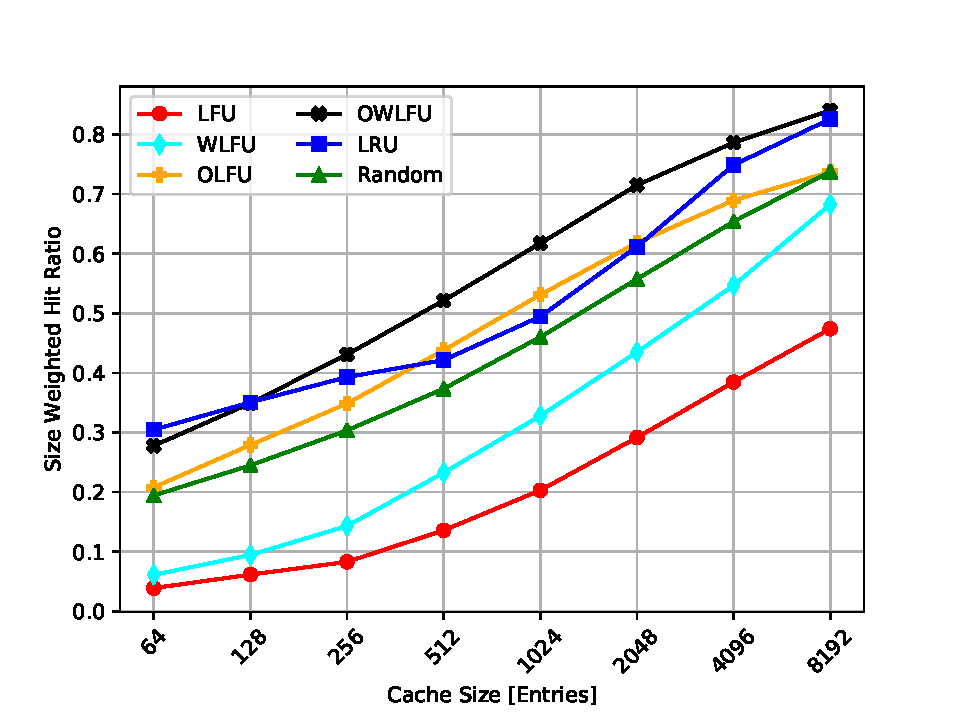
\includegraphics[width=0.33\textwidth]{weighted_hit_ratio_sf100.pdf}
\label{fig:weighted_hit_ratio_sf100}
}
\caption{Cache performance evaluation}
\label{fig:hit_ratio}
\end{figure*}


\subsection{Experimental Setup}
Table~\ref{tab:setup} presents the simulation parameters used to evaluate a two-level caching system as in Figure~\ref{fig:high_level_network}
We simulated the cache performance by emulating different cache policer slowdown factor ($SF$).
Note, that for a two-level caching scheme, $SF$ also represents the cache policer reaction time.
As performance metrics, we reported the cache hit ratio and the traffic size weighted hit ratio.
%The term slowdown factor ($SF$) refers to the cache policer reaction time.
%The slowdown factor is relative to the cache speed, i.e., a slowdown of 10$\times$ means that the cache policer is 10$\times$ slower than a cache access.
%The presented results were generated using the IXP New York to S\~ao Paulo data center trace~\cite{caida:19}.
The simulated traffic trace is the same as in~\S\ref{sec:traffic}.
To enable reproducibility, we open-sourced our codes\footnote{\url{https://github.com/engjefersonsantiago/Infinite_MT}.}.


\begin{table}[h]
	\centering
	\caption{Experimental Parameters}
	\label{tab:setup}
	\begin{tabular}{|l|l|}
		\hline
		\textbf{Parameter}       & \textbf{Value}   \\
		\hline
		Cache policy            & LRU, (O)(W)LFU, Random			    \\
		Cache Size              & 64 to \SI{8}{\kilo\nothing} entries  \\
		Slowdown Factor         & 1$\times$, 10$\times$, 100$\times$        \\
		\hline
	\end{tabular}
\end{table}

\subsection{Results}
Figure~\ref{fig:hit_ratio} presents the results for our experiments when no promotion policy is implemented.

As already reported in~\cite{Kim:09}, \textit{vanilla} LFU performs poorly with real-world network traffic.
Also, we confirmed the good performance of LRU-based policies with up-to-date data center traffic. 
The random policy achieves a relative good cache performance considering the small overhead for implementing it.
Random policy hit ratio lags behind the classic LRU by no more than 10 percentage points.

All modified versions of LFU significantly improve the cache performance compared to the \textit{vanilla} LFU.
WLFU observes a sharp increase in its hit ratio as the cache size increases.
OLFU observes a steady performance approaching the random hit ratio.
Indeed, OLFU introduces a pseudo-temporal variable to the LFU policy because it speculates that the promoted cache entry will be referenced in a near future. 
Last, OWLFU performs best in almost all scenarios.
This is nonetheless expected since it combines the strengths of OLFU and WLFU.

TODO: Check and run OPT simulations.

TODO: Comment the SF effect.

TODO: Evaluate the promotion policy.